\documentclass{article}
\usepackage{graphicx}
\topmargin=0.0in
\oddsidemargin=0.0in
\evensidemargin=0in 
\textwidth=6.5in
\marginparwidth=0.5in
\headheight=0pt 
\headsep=0pt
\textheight=9.0in
\newcommand\tab[1][3cm]{\hspace*{#1}}
 \begin{document}

 \begin{center}
 	 {
 	 	\large { SHUBHAM BARANWAL}
 	 }
 	
 \end{center}
 \hrule
 \begin{flushleft}
 	NIT Meghalaya, Bijni Complex, 		\hspace{1.7in}    		    Contact: 9436346271            \\
 	Laitumkhrah Shillong-793003  , 		\hspace{1.8in}		   e-mail id: shubhambaranwal2000@gmail.com\\
 	Meghalaya(India)     \\
\end{flushleft}

\vspace{-0.3in}

\begin{figure}[h]
	\hspace{4.4in}
	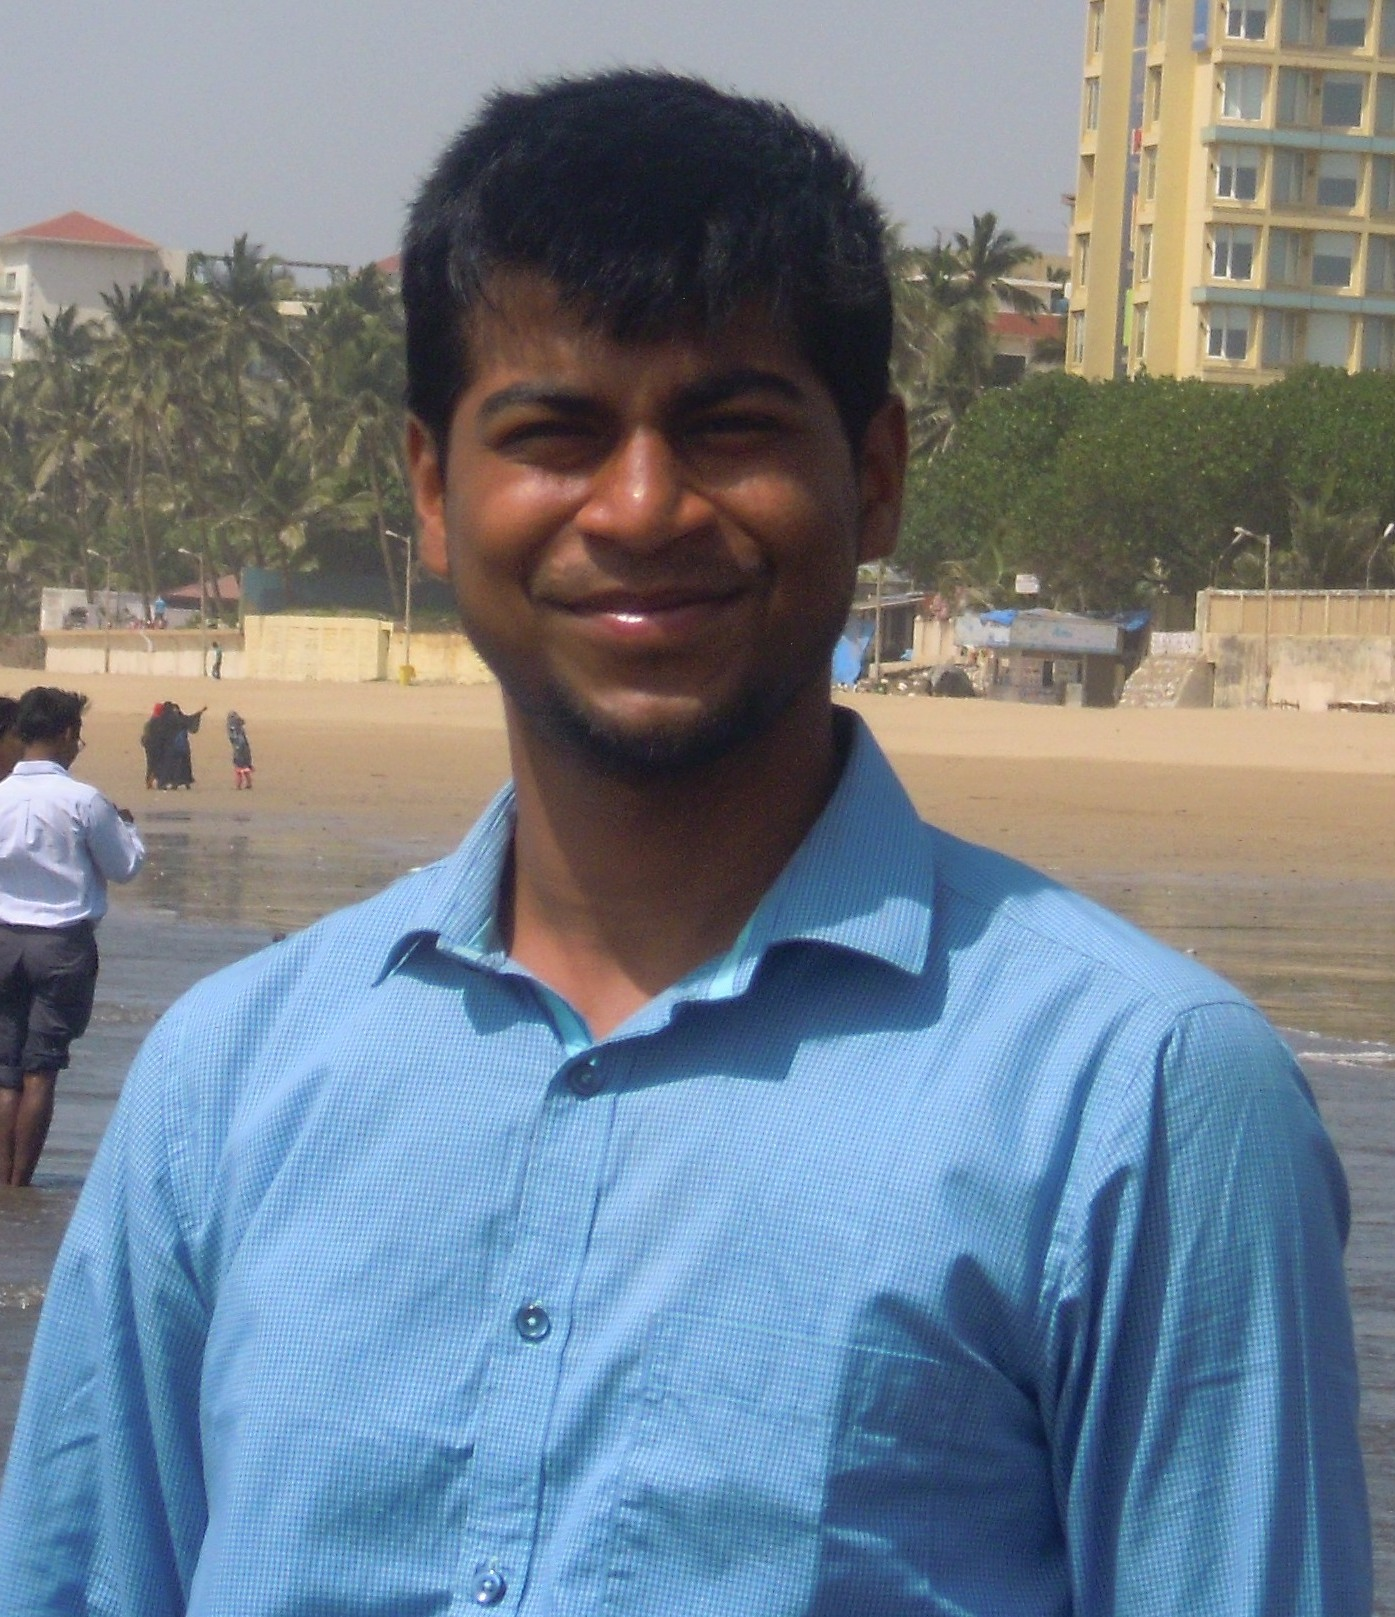
\includegraphics[width=90px]{shubham}
\end{figure}

%objective%

\begin{flushleft}
	\vspace{0.2in}
	\textbf{OBJECTIVE}
	
	\vspace{-0.20in}
	\hspace{1.4in}
	To enhance knowledge in the field of Embedded System and solve real-world \\
	\hspace{1.4in} problems
	
\end{flushleft}

 %  education %
 \begin{flushleft}
 	\vspace{0.3in}
 	\textbf{EDUCATION}
 	\hspace{0.1in}
 	\begin{tabular}{|c|c|c|c|c|}
 		\hline
 		Degree & School/College & Board/University & Passing Year & Percentage/CGPA   \\
 		\hline
 		B.tech & National Insitute & National Insitute & 2017 &8.34\\
 		E.E.E  & of Technology, Meghalaya & of Technology, Meghalaya & & (till 5th sem) \\
 		(pursuing) & & & &\\
 		\hline
 		AISSCE & Army Public School, & Central Board of & 2013 &90.83\\
 		(Class 12)  & Shillong & of Secondary Education & &\\
 		\hline
 		AISSE & Army Public School, & Central Board of & 2011 &10\\
 		(Class 10)  & Shillong & of Secondary Education & &\\
 		\hline
 		
 	\end{tabular}
 \end{flushleft}

% project %
\begin{flushleft} 
	\vspace{0.3in}
	\textbf{PROJECTS}
	\begin{enumerate}
		\vspace{-0.29in}
		\addtolength{\itemindent}{1.359in}
		\item  Autonomous Robot on Hazardous Waste Disposal Theme in e-YANTRA'15
		\item  Line Follower Robot using ATMEGA 16 Microcontroller
		\item Working on Smart Home Theme of Robotics and IOT Club, NIT
		Meghlaya
	\end{enumerate}
\end{flushleft}

\end{document}